\chapter{Bank Specification for serving memory requests}\label{ch4}
\noindent
A mixed criticality system consists of tasks from different criticality levels working on the same platform. A task may be 
of certain criticality level based on the safety of the system. Upto 5 levels of criticality levels are identified in 
automobile/avionics systems. For an automobile/avionics system, our goal is to ensure that no high critical task should miss 
their deadlines at the cost of any low critical task.
\newline
\newline
Let us consider an automobile system consisting of engine, fuel system, exhaust system, cooling system, lubrication system,
electrical system, transmission system, air-bag control system and the chassis. The chassis includes the brakes, tires, 
wheels, the suspension system and the body. When the system is in operating state, we have multiple messages coming from 
different applications. But some applications like the air-bag control system operates during emergency conditions to keep 
the system safe. So these messages are of higher criticality in order to ensure the safety of the system. 
\newline
\newline
We have considered a task as a set of memory requests. Each task can be executed in any criticality mode. Our task model is based on the power mode partitioning problem discussed in~\cite{DBLP:conf/vlsid/RayDC07} and the tenant mode allocation problem discussed in ~\cite{DBLP:conf/im/NandiBGB13, DBLP:journals/soca/NandiGBB17}. In this chapter, we will mainly focus on the memory bank design and memory requirements so that we can serve the memory 
requests of different critical tasks executing at different criticality levels.


\section{Memory Bank Requirements}\label{mrr}
Consider the memory hierarchy explained in the introductory chapters. The number of memory banks is unchangeable and needs to 
be specified at design time. 
\subsection{Problem Formulation}\label{pf1a}
\newtheorem{problem}{Problem}[section]
\begin{problem}
    Given a set of mixed critical tasks with different deadlines and with different memory requirements at different 
    criticality levels, the problem is to determine if the set of tasks can be served with a given number of memory banks such that all tasks finish execution within their 
    deadlines. 
\end{problem}
The above problem is introduced here with the help of an example.

\subsubsection{Motivating Example}\label{me}
Consider a set of tasks with some memory requests that are needed to be served within their deadlines. Each task is 
associated with a set of critical levels or modes in which the task can be executed, along with the number of parallel bank 
accesses required at a particular criticality level or mode and the percentage of task which gets completed on serving the 
memory request at that criticality level or mode. A set of tasks with different task parameters are given in Table \ref{tab1}. 
All tasks are assumed to have arrived at the same instant for memory access. We need to check whether we can serve all the 
memory requests at any criticality level within their deadlines on a memory with 12 banks.

\begin{table}[t]
 \begin{tabular}{|c|c|c|c|c|}\hline
 Task ID & Criticality Levels & Parallel Bank Access  & \% of task executed & Deadline \\ \hline
 1 & {$L_{11}$, $L_{12}$, $L_{13}$} & $L_{11}$ - 6 & $L_{11}$ - 25\% & 4 cycles \\
   &  & $L_{12}$ - 10 & $L_{12}$ - 35\% &  \\
   &  & $L_{13}$ - 0 & $L_{13}$ - 0\% & \\ \hline
 2 & {$L_{21}$, $L_{22}$, $L_{23}$} & $L_{21}$ - 5 & $L_{21}$ - 20\% & 5 cycles \\
   &  & $L_{22}$ - 10 & $L_{22}$ - 30\% & \\
   &  & $L_{23}$ - 0 & $L_{23}$ - 0\% & \\ \hline
 3 & {$L_{31}$, $L_{32}$, $L_{33}$, $L_{34}$} & $L_{31}$ - 0 & $L_{31}$ - 0\% & 6 cycles \\
   &  & $L_{32}$ - 4 & $L_{32}$ - 15\% & \\
   &  & $L_{33}$ - 8 & $L_{33}$ - 25\% & \\
   &  & $L_{34}$ - 12 & $L_{34}$ - 40\% & \\ \hline 
 \end{tabular}
\caption{Task Specifications}
\label{tab1}
\end{table}

\noindent
Intuitively, if we consider the maximum bank required by each task in any criticality mode, then we see that a memory 
with 32 banks can run all the tasks in parallel and hence will be able to schedule all the tasks within their deadlines.
But our system may not always have huge amount of resources to execute all the tasks in parallel. So we need to schedule the 
tasks in such a way that we use our resources efficiently as well as we can meet the task deadlines. 

\noindent 
Given the above set of tasks and a memory with say 12 banks, we need to answer whether all these tasks can complete 
their execution within their deadlines. The above decision problem can be formulated using the following conventions- 

\noindent
\newtheorem{defn}{Definition}[section]

\begin{defn}
$i^{th}$ task $\tau_{i}$ is defined as -
\newline
\newline
$\tau_{i} = (L_{i}, B_{i}, E_{i}, D_{i})$
\newline
\newline
where, $L_{i}$ $\in$ $\mathbb{Z^{+}}$, denoting j criticality levels which task $\tau_{i}$ can exibit,
\newline
\newline
$B_{i}$ : $L_{i}$ $\rightarrow$ $\mathbb{N}$, $B_{i}$ denotes the number of parallel bank access that 
$\tau_{i}$ exhibits at each criticality level in $L_{i}$,
\newline
\newline
$E_{i}$ : $L_{i}$ $\rightarrow$ $\mathbb{R}$, $E_{i}$ denotes the percentage of total task that can be completed by $\tau_{i}$ at each criticality level in  $L_{i}$.
\newline
\newline
$D_{i}$ $\in$ $\mathbb{Z^{+}}$, denotes the deadline of $i^{th}$ task $\tau_{i}$
\newline
\end{defn}

\noindent
The problem is to synthesize a schedule for the tasks at each cycle, with each task assigned to one of its criticality levels, 
such that all tasks finish execution by their respective deadlines. A feasible schedule to the task set (a solution to the 
above problem) must therefore, satisfy the following conditions:
\begin{itemize}
 \item Condition 1: In every cycle a task will execute in exactly one of its criticality levels.
\item Condition 2: A task must complete 100\% of its execution before its deadline.
\item Condition 3: At any cycle the total number of banks accessed by all the executing tasks must be less than or equal to the 
number of banks available to the system.
\end{itemize}

\noindent
We now attempt to characterize the hardness of the problem. As above, we are given a set $T$ of tasks, each having deadline 
d(t) $\in$ $\mathbb{Z^{+}}$, a number m $\in$ $\mathbb{Z^{+}}$ of banks, number r $\in$ $\mathbb{Z^{+}}$ of resource 
requirements (number of parallel bank access) of each task in each cycle depending on its criticality level, resource bounds 
m in each cycle, resource requirements $B_{i}(t)$ of $i^{th}$ task, 
0 $\leq$ $B_{i}(t)$ $\leq$ m. The problem of finding a schedule for the above is NP-complete. The problem is definitely in NP 
since we can verify in polynomial time if a given schedule satisfies the requirement on bank access and task deadline. 
To show that our problem is NP-hard, we present below a polynomial time reduction from the partition problem~\cite{wiki:xxx7} 
to our problem.
Given an instance $\alpha$ of partition problem, we will generate an instance of our problem $\sigma$ such that if $\alpha$
can be partitioned into $p$ partitions, $\sigma$ can also be scheduled over $p$ cycles (where $p$ denotes the maximum largest 
deadline value) with m banks.
\newline
\newline
Our problem is a variant of the resource constrained problem~\cite{garey2002computers} with resource bounds equal to m and 
each task having individual task deadlines. A task can be identified as a set of subtasks executing with different amount of 
resources. In each cycle, we need to generate a partition consisting of subtasks such that the sum of resources at every cycle 
is atmost m and each task can complete 100\% of its execution within their individual deadlines. 
\newline
\newline
Our problem instance $\alpha$ consists of a set of elements, represented by $E_{i}$, i varies from 1 to $|\alpha|$. 
Each element of $E_{i}$ is again a set of tuples - a number and a cost associated with that number. So, each $E_{i}$ consists 
of tuples of the form ($n_{ij}$,$C_{ij}$), where j varies from 1 to $|E_{i}|$. Our objective is to partition $\alpha$ into 
p partitions such that each partition $p_{k}$ contains atmost one number $n_{ij}$ from every $E_{i}$ so that the sum of the 
numbers in each partition is atmost m and the sum of the costs corresponding to all the selected numbers of $E_{i}$ over p 
partitions is atleast 100. Each element $E_{i}$ again can be selected for some definite number of partitions.  
On selecting the $j^{th}$ number from the $i^{th}$ element in the set $\alpha$, a subtask of $i^{th}$ task is selected whose bank 
requirement is the $j^{th}$ number that is selected and the cost associated with the number, $C_{ij}$, is the percentage of 
execution of $i^{th}$ task at $j*{th}$ criticality level with $n_{ij}$ number of parallel bank access. In every partition, 
$p_{k}$, the sum of all the numbers must be atleast m. When the total cost of $i^{th}$ element is greater than or equal to 100 
over all p partitions, then $i^{th}$ task gets completed. On getting a partition at every iteration with the above 
constraints, we actually get a schedule for our problem. So if $\alpha$ can be partitioned into p partitions, $\sigma$ is 
schedulable over p cycles with m banks.
Again, the converse is also true.
Suppose that our problem can complete execution of all the tasks over p cycles. We construct a schedule $\sigma$ of our 
problem such that over p cycles, $\sigma$ can schedule all the tasks within their deadlines with m number of resources (banks)
in each cycle. For $i^{th}$ task executing in $j^{th}$ criticality level in the schedule $\sigma$, a number from the $i^{th}$ 
element of the multiset $\alpha$ is selected. The total number of banks accessed in every cycle in the schedule $\sigma$ is 
atmost m, ensuring the sum of the numbers in every partition cannot exceed m. Completion of $i^{th}$ task in the schedule 
$\sigma$ over all p cycles is equivalent to the sum of costs corresponding to every number selected from the $i^{th}$ element 
in $\alpha$ over all p partitions to be atleast 100. A schedule $\sigma$ exists, denoting that all the tasks can be completed 
in p cycles with m banks. This implies $\alpha$ can also be partitioned into p partitions. Thus, the problem of deciding if a schedule exists for all the tasks with individual task deadlines over m banks in every cycle is
NP-complete.



\subsection{Constraint Formulation}\label{cf}
The decision problem introduced above can be stated with the following constraints.
We are given a number of banks $z$. 
To formulate the above problem we define a decision variable say $f_{ijk}$.
\newline
\begin{align*}
 f_{ijk} &=
 \begin{cases}
  1	& \text{if $i^{th}$ task executes in $j^{th}$ criticality level in $k^{th}$ cycle} \\
  0	& \text{otherwise}
 \end{cases}
\end{align*}
\newline
The above decision problem can be expressed with  a set of constraints which are as follows. From Condition 1, we get that for all cycles, a task can execute in exactly one of its criticality level. Therefore, for each task $\tau_i$,
\begin{equation} 
\sum_{j = 1}^{|L_{i}|} f_{ijk} = 1, \forall k, 1 \leq k \leq D_i
\end{equation}
\newline
From Condition 2, we get that all tasks should complete 100\% execution before their deadlines. The percentage of task that 
gets completed at the last cycle may exceed 100. So we have used '$\geq$' instead of 
'='. Therefore, 
\begin{equation}
\sum_{k = 1}^{D_{i}} \sum_{j = 1}^{|L_{i}|} E_{i}(L_{ij}) * f_{ijk} \geq 100, \forall i, 1 \leq i \leq n
\end{equation}
\newline
Here, $E_{ij}(L_{ij})$ denotes the percentage of $i^{th}$ task that can be executed at criticality level j, $n$ denotes the total 
number of tasks. 
From Condition 3, we get that at any cycle the total number of banks required by all the tasks executing at that cycle must be
atmost $z$.
\begin{equation}
\sum_{i = 1}^{n} \sum_{j = 1}^{|L_{i}|} B_{i}(L_{ij}) * f_{ijk} \leq z, \forall k, 1 \leq k \leq D_i
\end{equation}
\newline
where $n$ denotes the number of tasks and $z$ denotes the number of banks available to the system. Here, $B_{i}(L_{ij})$ 
denotes the parallel bank access required by $i^{th}$ task at criticality level $j$.
\newline
In the above decision problem the value of $z$ is 12. 
For z = 12, we check whether all the tasks will meet their deadlines.
We get a total of (4 + 5 + 6) = 15 constraints from Condition 1 for different tasks at each cycle k.
\newline
\begin{equation}
 f_{111} + f_{121} + f_{131} = 1
\end{equation}
\begin{equation}
 f_{211} + f_{221} + f_{231} = 1
\end{equation}
\begin{equation}
 f_{311} + f_{321} + f_{331} + f_{341} = 1
\end{equation}
\begin{equation}
 f_{112} + f_{122} + f_{132} = 1
\end{equation}
\begin{equation}
 f_{212} + f_{222} + f_{232} = 1
\end{equation}
\begin{equation} 
 f_{312} + f_{322} + f_{332} + f_{342} = 1
\end{equation}
\begin{equation}
 f_{113} + f_{123} + f_{133} = 1
\end{equation}
\begin{equation}
 f_{213} + f_{223} + f_{233} = 1
\end{equation}
\begin{equation}
 f_{313} + f_{323} + f_{333} + f_{343} = 1
\end{equation}
\begin{equation}
 f_{114} + f_{124} + f_{134} = 1
\end{equation}
\begin{equation}
 f_{214} + f_{224} + f_{234} = 1
\end{equation}
\begin{equation}
 f_{314} + f_{324} + f_{334} + f_{344} = 1
\end{equation}
\begin{equation}
 f_{215} + f_{225} + f_{235} = 1
\end{equation}
\begin{equation}
 f_{315} + f_{325} + f_{335} = 1
\end{equation}
\begin{equation}
 f_{316} + f_{626} + f_{336} = 1
\end{equation}
\newline
Again, from Condition 2, we get 3 constraints for different tasks.
\newline
\begin{equation}
 25 * (f_{111} + f_{112} + f_{113} + f_{114}) + 35 * (f_{121} + f_{122} + f_{123} + f_{124}) \geq 100 
\end{equation}
\begin{equation}
 20 * (f_{211} + f_{212} + f_{213} + f_{214} + f_{215}) + 30 * (f_{221} + f_{222} + f_{223} + f_{224} + f_{225}) \geq 100
\end{equation}
\begin{equation}
\begin{split}
 15 * (f_{321} + f_{322} + f_{323} + f_{324} + f_{325} + f_{326}) + 25 * (f_{331} + f_{332} + f_{333} + f_{334} + f_{335} + 
 f_{336}) \\
 + 40 * (f_{341} + f_{342} + f_{343} + f_{344} + f_{345} + f_{346}) \geq 100
 \end{split}
\end{equation}
\newline
Again, from Condition 3, we get 6 constraints for different clock cycle k.
\newline
\begin{equation}
 6 * f_{111} + 10 * f_{121} + 5 * f_{211} + 10 * f_{221} + 4 * f_{321} + 8 * f_{331} + 12 * f_{341} \leq 12
\end{equation}
\begin{equation}
 6 * f_{112} + 10 * f_{122} + 5 * f_{212} + 10 * f_{222} + 4 * f_{322} + 8 * f_{332} + 12 * f_{342} \leq 12
\end{equation}
\begin{equation}
 6 * f_{113} + 10 * f_{123} + 5 * f_{213} + 10 * f_{223} + 4 * f_{323} + 8 * f_{333} + 12 * f_{343} \leq 12
\end{equation}
\begin{equation}
 6 * f_{114} + 10 * f_{124} + 5 * f_{214} + 10 * f_{224} + 4 * f_{324} + 8 * f_{334} + 12 * f_{344} \leq 12
\end{equation}
\begin{equation}
 5 * f_{215} + 10 * f_{225} + 4 * f_{325} + 8 * f_{335} + 12 * f_{345} \leq 12
\end{equation}
\begin{equation}
 4 * f_{326} + 8 * f_{336} + 12 * f_{346} \leq 12
\end{equation}
\newline
Solving these set of constraints, we get that the above tasks cannot meet their deadlines on a memory with bank size 12.  
So the above set of tasks is not schedulable for a memory with 12 banks. This leads us to two questions which are discussed 
in the following sections-
\begin{description}

\item {1}: The maximum number of tasks that can be executed at different criticality levels within their deadlines on a 
memory with z banks.

\item {2}: The minimum number of banks required to design a system consisting of tasks with different criticality levels 
and different deadlines.

\end{description}

\section{Task Maximization Problem}\label{tmp}
The above decision problem leads to the question that if a set of tasks is not schedulable with a bank of particular size, 
then what is the maximum number of tasks which can be schedulable for the set of tasks with the above parameters.

\subsection{Problem Formulation}\label{pf}
\begin{problem}
Given a set of tasks with different sets of criticality levels along with number of parallel bank access required at each 
criticality level, and percentage of task completed if executed at that criticality level. Each task is also associated with 
a deadline. We are given a memory with z number of banks, we need to find out the maximum number of tasks that can complete 
their execution within their deadlines. 
\end{problem}
We explain the task maximization problem with the set of tasks in Table \ref{tab1}. 
% Using a similar reduction from the multi-set partitioning problem, we can show that this is NP-complete as well.
% The same set of conditions as in the earlier need to be satisfied in this case as well. problem are as follows:
% 
% \newline
% \newline
% Condition 1: In every cycle a task will execute in exactly one of its criticality level.
% \newline
% \newline
% Condition 2: A task must complete 100\% of its execution before its deadline.
% \newline
% \newline
% Condition 3: At any cycle the total number of banks accessed by all the executing tasks must be less than or equal to the 
% number of banks available to the system.
% \newline
% 
% 
% \subsection{Hardness Characterisation of the problem}\label{hcpm}
% \begin{theorem}
%  Given a set T of tasks, each having length l(t) $\in$ $\mathbb{Z^{+}}$, with deadline d(t) $\in$ $\mathbb{Z^{+}}$, 
%  number m $\in$ $\mathbb{Z^{+}}$ of banks, number r $\in$ $\mathbb{Z^{+}}$ of resource requirements (number of parallel bank 
%  access) of each task, resource bounds m in each cycle, resource requirements $B_{i}(t)$ of $i^{th}$ task, 
%  0 $\leq$ $B_{i}(t)$ $\leq$ m, for each task t and resource bound (number of banks available) is m in each cycle - Can we 
%  schedule the maximum K number of tasks within their deadlines over p cycles with a resource bound of m in each cycle.
% \end{theorem}
% \noindent
% The problem is NP-hard.
% 
% \newline
% \newline
 The problem is NP-hard.
 To show that our problem is NP-hard, we give a polynomial time reduction from partition problem~\cite{wiki:xxx7} to our 
 problem.
 Given a instance $\alpha$ of partition problem, we will generate an instance of our problem $\sigma$ such that if the gain 
 over $\alpha$ is atleast K over p partitions, $\sigma$ can also ensure completion of K tasks over p cycles.
 Our problem is a variant of scheduling to minimize weighted completion time~\cite{garey2002computers} with resource bounds 
 equal to m in each cycle. A task instance in our problem can be identified as a set of subtasks executing with different 
 amount of resources. In each cycle, we need to generate a partition consisting of subtasks such that the sum of resources at 
 every cycle is atmost m and atleast K tasks can be completed within their individual deadlines. We associate weights w(t) to 
 each task such that on completion of each task a weight w(t) is added to the total cost of the system. We need to guarantee 
 that the total weight associated with the system must be atleast K * w(t). 
 \newline
 \newline
 Our problem instance $\alpha$ consists of a set of elements, represented by $E_{i}$, i varies from 1 to $|\alpha|$. 
Each element of $E_{i}$ is again a set of tuples - a number and a cost associated with that number. So, each $E_{i}$ consists 
 of tuples of the form ($n_{ij}$,$C_{ij}$), where j varies from 1 to $|E_{i}|$. We need to partition $\alpha$ into 
 p partitions such that each partition $p_{k}$ contains atmost one number $n_{ij}$ from every $E_{i}$ so that the sum of the 
 numbers in each partition is atmost m and the sum of the costs corresponding to all the selected numbers of $E_{i}$ over p 
 partitions is atleast 100. Our objective is to guarantee that the number of elements $E_{i}$ whose cost over p partitions has 
 exceeded 100 is atleast K, ie, we have a gain of atleast K. Each element $E_{i}$ again can be selected for some definite 
 number of partitions. 
 \newline
 \newline
 On selecting $j^{th}$ number from $i^{th}$ element in the set $\alpha$, a subtask of $i^{th}$ task is selected whose bank 
 requirement is the $j^{th}$ number that is selected and the cost associated with the number, $C_{ij}$, is the percentage of 
 execution of $i^{th}$ task at $j^{th}$ criticality level with $n_{ij}$ number of parallel bank access. In every partition, 
 $p_{k}$, the sum of all the numbers must be atleast m. When the total cost of $i^{th}$ element is greater than or equal to 100 
 over all p partitions, then $i^{th}$ task gets completed and 1 is added to the gain function. If $\alpha$ results in a gain of
 atleast K over p partitions, then $\sigma$ can also ensure completion of K tasks over p cycles with a total weight of atleast 
 K * w(t) over p cycles.
 \newline
 \newline
 Again, the converse is also true.
 \newline
 \newline
 Suppose that our problem can complete execution of K tasks over p cycles. We construct a schedule $\sigma$ of our 
 problem such that over p cycles, $\sigma$ can schedule K tasks within their deadlines with m number of resources (banks)
 in each cycle. For $i^{th}$ task executing in $j^{th}$ criticality level in the schedule $\sigma$, a number from the $i^{th}$ 
 element of the multiset $\alpha$ is selected. The total number of banks accessed in every cycle in the schedule $\sigma$ is 
 atmost m, ensuring the sum of the numbers in every partition cannot exceed m. Completion of $i^{th}$ task in the schedule 
 $\sigma$ over all p cycles is equivalent to the sum of costs corresponding to every number selected from the $i^{th}$ element 
 in $\alpha$ over all p partitions to be atleast 100. Now, completion of K tasks over p cycles in $\sigma$ means the 
 total cost to the system is K * w(t). Therefore, number of elements in $\alpha$ whose sum is atleast 100 is K. So, $\alpha$ 
 has a gain of K over p partitions.
 \newline
 \newline
 Therefore, maximum task execution over m banks with individual task deadlines and a resource bound of m in every cycle is
 NP-hard.

\subsection{Maximum Task Execution : Constraint Formulation}
We introduce a new decision variable $C_{i}$ to keep track of the task completion. $C_i$ marks the completion of task $T_i$.
\begin{align*}
 C_{i} &=
 \begin{cases}
  1	& \text{$i^{th}$ task $T_{i}$ has completed 100\% of the task} \\
  0	& \text{otherwise}
 \end{cases}
\end{align*}
\newline
We define the task maximization problem using Integer Linear Programming (ILP) as follows -
\newline
\begin{center}
 Maximize $\sum_{i = 1}^{n} C_{i}$, subject to
 \end{center}
For each task $\tau_i$,
 \begin{equation}\label{eq1}
\sum_{j = 1}^{|L_{i}|} f_{ijk} \leq 1, \forall k, 1 \leq k \leq D_{i}
\end{equation}
\newline
\begin{equation}\label{eq2}
\sum_{k = 1}^{D_{i}} \sum_{j = 1}^{|L_{i}|} E_{i}(L_{ij}) * f_{ijk} \geq 100 * C_i, \forall i, 1 \leq i \leq n 
\end{equation}
\newline
\begin{equation}\label{eq3}
\sum_{i = 1}^{n} \sum_{j = 1}^{|L_{i}|} B_{i}(L_{ij}) * f_{ijk} \leq z, \forall k,1 \leq k \leq D_i
\end{equation}
\newline
From Condition 1, we get that at any cycle k, a task can exist in any one of its criticality level. Therefore, Eqn. \ref{eq1}
holds from Condition 1. Similarly, Eqn. \ref{eq2} is obtained from Condition 2. Hence, if any task say T1 has completed 
its 100\% execution, then the flag $C_{1}$ is set and the Condition 2 holds. If $C_{1}$ flag is 0, meaning that the task T1 
has not yet completed its 100\% execution. So, Condition 2 holds in both the cases. From Condition 3, we get Eqn. \ref{eq3} 
where the number of banks required must be less than or equal to z at every cycle. 
Formulating the above equations in the form of constraints on the set of tasks in Table \ref{tab1} for the task maximization 
problem, we get a total of 18 constraints from Condition 1, 3 constraints from Condition 2 and 6 constraints from Condition 3.
Solving the above set of 27 constraints, we get the answer for the maximum number of tasks that can be executed and also 
the schedule for the task maximization problem. Table \ref{tab3} in the Results section of this chapter shows the maximum number of tasks that can be schedulable for a given set of tasks and a given set of 
system resources.


\section{Bank Minimization Problem}\label{bmp}
\noindent
The decision problem discussed in the first section of this chapter can only tell us if a set of tasks with a fixed number of 
banks and with certain task parameters is schedulable or not. But if no feasible schedule exists then we need to know the 
minimum number of banks required to schedule a given set of tasks.

\subsection{Problem Formulation}\label{pf1}
\begin{problem}
    Given a set of tasks with different deadlines. Each task is associated with different criticality levels, number of 
    parallel bank access at that criticality level and percentage of task executed on serving those memory requests at that 
    criticality level. We need to answer the minimum number of banks required to execute all the tasks within their deadlines.
\end{problem}
This problem can be formulated in a similar way like the above decision problem discussed in the first section with minor 
changes in the constraints and the objective function.

\subsection{Hardness Characterization of the problem}\label{hcp}
\noindent
\begin{problem}
 Given a set $T$ of tasks, each having length l(t) $\in$ $\mathbb{Z^{+}}$, with deadline d(t) $\in$ $\mathbb{Z^{+}}$, 
 number r $\in$ $\mathbb{Z^{+}}$ of resource requirements (number of parallel bank access), resource requirements $B_{i}(t)$ 
 of $i^{th}$ task, for each task $t$ - Can we get the minimum number of banks K required to schedule all the tasks $t$ $\in$ $T$ 
 with resource bound of K in each cycle over a period of p cycles.
\end{problem}
\noindent
It can be shown that this problem is NP-hard using a similar reduction technique as in the case of the decision problem.
% 
% \newline
% \newline
% To show that our problem is NP-hard, we give a polynomial time reduction from partition problem~\cite{wiki:xxx7} to our 
% problem.
% Given a instance $\alpha$ of partition problem, we will generate an instance of our problem $\sigma$ such that if $\alpha$
% can be partitioned into p partitions with a minimum sum of K in each partition, $\sigma$ can also be scheduled over p cycles 
% with K banks. It can be shown 
% \newline
% \newline
% Our problem is a variant of the resource constrained problem~\cite{garey2002computers} with resource bounds equal to K and 
% each task having individual task deadlines. A task can be identified as a set of subtasks executing with different amount of 
% resources. In each cycle, we need to generate a partition consisting of subtasks such that the sum of resources at every cycle 
% is at most K and each task can complete 100\% of its execution within their individual deadlines. 
% \newline
% \newline
% Our problem instance $\alpha$ consists of a set of elements, represented by $E_{i}$, i varies from 1 to $|\alpha|$. 
% Each element of $E_{i}$ is again a set of tuples - a number and a cost associated with that number. So, each $E_{i}$ consists 
% of tuples of the form ($n_{ij}$,$C_{ij}$), where j varies from 1 to $|E_{i}|$. Our objective is to partition $\alpha$ into 
% p partitions such that each partition $p_{k}$ contains atmost one number $n_{ij}$ from every $E_{i}$ so that the sum of the 
% numbers in each partition is atmost K and the sum of the costs corresponding to all the selected numbers of $E_{i}$ over p 
% partitions is atleast 100. Each element $E_{i}$ again can be selected for some definite number of partitions.  
% \newline
% \newline
% On selecting $j^{th}$ number from $i^{th}$ element in the set $\alpha$, a subtask of $i^{th}$ task is selected whose bank 
% requirement is the $j^{th}$ number that is selected and the cost associated with the number, $C_{ij}$, is the percentage of 
% execution of $i^{th}$ task at $j*{th}$ criticality level with $n_{ij}$ number of parallel bank access. In every partition, 
% $p_{k}$, the sum of all the numbers must be atleast K. When the total cost of $i^{th}$ element is greater than or equal to 100 
% over all p partitions, then $i^{th}$ task gets completed. On getting a partition at every iteration with the above 
% constraints, we actually get a schedule for our problem. So if $\alpha$ can be partitioned into p partitions, $\sigma$ is 
% schedulable over p cycles with K banks.
% \newline
% Again, the converse is also true.
% \newline
% \newline
% Suppose that our problem can complete execution of all the tasks over p cycles. We construct a schedule $\sigma$ of our 
% problem such that over p cycles, $\sigma$ can schedule all the tasks within their deadlines with a minimum of K number of 
% resources (banks) in each cycle. For $i^{th}$ task executing in $j^{th}$ criticality level in the schedule $\sigma$, a number 
% from the $i^{th}$ element of the multiset $\alpha$ is selected. The total number of banks accessed in every cycle in the 
% schedule $\sigma$ is atmost K, ensuring the sum of the numbers in every partition cannot exceed K. Completion of $i^{th}$ task 
% in the schedule $\sigma$ over all p cycles is equivalent to the sum of costs corresponding to every number selected from the 
% $i^{th}$ element in $\alpha$ over all p partitions to be atleast 100. A schedule $\sigma$ exists, denoting that all the tasks 
% can be completed in p cycles with K banks. This implies $\alpha$ can also be partitioned into p partitions.
% \newline
% \newline
% Therefore, minimum number of banks required to schedule a set of tasks with individual deadlines is NP-hard.

\subsection{Constraint Formulation}\label{cfp}
\noindent
Let z be the number of memory banks and n be the number of tasks to be executed at a particular instant. Our problem can be 
expressed using Integer Linear Programming as - 
\newline
\begin{center}
 Minimize z subject to
 \end{center}
 For each task $\tau_i$,
\begin{equation}
\sum_{j = 1}^{|L_{i}|} f_{ijk} \leq 1, \forall k, 1 \leq k \leq D_{i}
\end{equation}
\newline
\begin{equation}
\sum_{k = 1}^{D_{i}} \sum_{j = 1}^{|L_{i}|} E_{i}(L_{ij}) * f_{ijk} \geq 100, \forall i, 1 \leq i \leq n
\end{equation}
\newline
\begin{equation}
\sum_{i = 1}^{n} \sum_{j = 1}^{|L_{i}|} B_{i}(L_{ij}) * f_{ijk} \leq z, \forall k, 1 \leq k \leq D_i
\end{equation}
\newline
By applying the above constraints on the tasks in Table \ref{tab1}, we require a memory with atleast 15 banks to complete the 
tasks within their deadlines. A memory with bank size less than 15 will fail to meet all the task deadlines. 
Table \ref{tab2} in the Results section of this chapter shows some sets of critical tasks and corresponding minimum number of 
banks required to execute all the tasks within their deadlines.


\section{Bank Minimization using Binary Search}\label{RMBS}
\noindent
We know that for the bank minimisation problem, the solution for the minimum number of banks will lie in between 1 to M where
M is the sum of maximum number of banks required by any task at its any criticality level. For the tasks in Table \ref{tab1},
the optimal solution will lie somewhere in between 1 to (10 + 10 + 12) = 32, (the sum of the maximum number of banks of each
task). Using Integer Linear Programming to minimise or 
maximize the objective function requires a lot of computation cost for a very large problem with many constraints. Also it 
increases the search space and time complexity of the problem. We can significantly decrease the computational cost and space 
complexity of the problem by applying a binary search on the search space. Since, we know that a solution will always 
exist in between 1 and M, therefore, instead of solving for the minimum number of banks we can apply a binary search on the value 
of z and check if the solution is optimal for that value of z. The solution is a straight adaptation of the one in~\cite{DBLP:conf/vlsid/RayDC07}. 

\subsection{Binary Search Algorithm on the bank minimization problem}\label{bsa}
Algorithm \ref{alg1}, \ref{alg2} and \ref{alg3} give a description of our binary search algorithm on bank minimisation 
problem.
\begin{algorithm}
 \caption{Bank Minimization using binary search}
  \begin{algorithmic}[1]
   \Function {binsrch}{$n ,TaskList$} \Comment $n$ denotes the number of tasks, $Tasklist$ is the list of $n$ tasks along 
    with all the task parameters
    \State min = 1 \Comment Minimum number of banks can be 1
     \State max = compute\_max\_banks($n, TaskList$)\Comment find upper bound for the number of banks required
      \State result = -1 
      \While {(max $>$ min) and (result $\neq$ 0)}
       \State mid = (min + max)/2
        \State result = check\_feasibility($mid,n,TaskList$)\Comment a Function which returns positive value if mid is greater than optimal solution and negative value if mid is less than optimal
         \If {result $<$ 0}
          \State min = mid + 1
           \ElsIf {result $>$ 0}
            \State max = mid -1
               \EndIf
                \EndWhile
                 \State return mid
                 \EndFunction
  \end{algorithmic}
 \label{alg1}
\end{algorithm}

\begin{algorithm}
\caption{compute maximum number of banks required}
 \begin{algorithmic}[1]
   \Function {compute\_max\_banks}{$n, TaskList$}\Comment calculates the upper bound for the number of banks required
    \State max = 0
     \For {$i$ = $1$ to $n$}
      \For {$j$ = $1$ to length(TaskList[i].Criticality\_Level)}
       \If {TaskList[i].Bank[j] $>$ max} 
        \State max = TaskList[i].Bank[j]
         \EndIf
          \EndFor
           \EndFor
            \State return max   
             \EndFunction
  \end{algorithmic}
 \label{alg2}
\end{algorithm}

\begin{algorithm}
 \caption{check feasibility of the solution}
  \begin{algorithmic}[1]
   \Function {check\_feasibility}{$val,n,TaskList$}
    \For {$i$ = 1 to $n$}
     \For {$j$ = 1 to length($TaskList[i].Criticality$)}
      \For {$k$ = 1 to $TaskList[i].Deadline$}
       \State Apply the constraints for a bank of size val \Comment call LpSolver and apply the constraints for a bank of size val 
        \EndFor
         \EndFor
          \EndFor
           \State result = assert\_optimal()\Comment check if the status of the solution is optimal for a bank of size val 
            \State return result \Comment result $<$ 0 for infeasible solution, result $>$ 0 for feasible solution, result $equal$ 0 for optimal solution 
             \EndFunction
  \end{algorithmic}
 \label{alg3}
\end{algorithm}

\subsection{Complexity Analysis}\label{cabs}
Unlike conventional procedures for getting the minimum number of banks required to schedule a set of tasks within their 
deadlines, binary search reduces the search space by half at each step. Thus, in the worst case, number of function calls to 
check the feasibility of the solution is equal to the number of times we calculate the mid in the binary search problem. The 
check\_feasibility() function calls the decision problem to check for the optimality of the solution. It checks for which 
value of mid our solution is optimal (the point where the function returns 0). This is equivalent to finding 0 in an array of 
sorted numbers by binary search. For a problem of size $n$, our solution is logarithmic in $n$, as is the usual case with binary search. 
So the search space explored on which the decision problem is called is smaller, corresponding to the mid 
values, and hence space complexity of the problem reduces significantly. Moreover, since the decision problem is called 
log(n) times in the worst case, the space required by the decision problem can be evaluated as the peak requirement among all the space 
required by the log(n) function calls. As these log(n) function calls are called individually, so the space allocated at each 
function call is significantly much lower than that allocated for solving the bank minimization problem. On the other hand, we apply ILP to get an answer to the minimization problem on the entire search space of the problem. 
Though the solver uses some heuristics to minimize the search space, the space complexity is larger.
A comparative study of the space complexities of binary search in contrast to our ILP based solution on different task sets is 
shown in the results section of this chapter.


\subsection{Correctness of binary search based optimal solution generation}\label{cabsos}
We wish to prove here that our approach always generates a valid optimal solution for the minimum number of banks.
Let P(n) be the assertion that binsrch works correctly for inputs where right - left = n. If we can prove that P(n) is true 
$\forall$ n, then we know that binsrch will definitely give us the value of n for which the optimal solution exists. 
\newline
\newline
Base Case. In the above example when n = 0, min = max = m (say). Since we have assumed that the iteration would continue 
till the optimal solution is found between min and max, it must be the case that x = 0, ie, the optimal solution lies at m,
and the function will return m, a value in between min and max.
\newline
\newline
Inductive Step. We assume that binsrch works as long as left - right $\leq$ k. Our goal is to prove that it works on an input 
where left - right = k + 1. There are three cases, where x = 0, where x $<$ 0 and where x$>$ 0.
\newline
\newline
Case x = 0, the optimal solution lies at m. Clearly the function works correctly.
\newline
\newline
Case x $>$ 0, the optimal solution lies at some value smaller than x. We know that natural numbers between min and max are in 
ascending order, hence they are sorted. Therefore, the optimal solution must be found between min and m - 1. The n for the 
next iteration is n = m - 1 - left = ⌊(left + right)/2⌋ - 1 - left. (Note that ⌊x⌋ is the floor of x, which rounds it down 
toward negative infinity.) If left + right is odd, then n = (left + right - 1)/2 - 1 - left = (right - left)/2 - 1, which is 
definitely smaller than right - left. If left + right is even then n = (left + right)/2 - 1 - left = (right - left)/2, which 
is also smaller than k + 1 = right - left because right - left = k + 1 $>$ 0. So the recursive call must be to a range of a 
that is between 0 and k cells, and must be correct by our induction hypothesis.
\newline
\newline
Case x $<$ 0. The optimal solution lies at some value greater than x. This is more or less symmetrical to the previous case. 
We need to show that r - (m + 1) $\leq$ right - left. We have r - (m + 1) - l = right - ⌊(left + right)/2⌋ - 1. If right + left is 
even, this is (right - left)/2 - 1, which is less than right - left. If right + left is odd, this is 
right - (left + right - 1)/2 - 1 = (right - left)/2 - 1/2, which is also less than right - left. Therefore, the iterative call 
is to a smaller range of the array and can be assumed to work correctly by the induction hypothesis. We can thus conclude that binsrch is correct.

 \section{Results}\label{res}
 This section presents different results generated on different set of tasks. 
  
 \begin{table}[!htb]
 \begin{tabular}{|c|c|c|c|c|c|}\hline
 {\bf Task ID} & {\bf Criticality} & {\bf Parallel Bank}  & {\bf Percentage of} & {\bf Deadline} & {\bf Minimum Bank} \\
         & {\bf Level} & {\bf Access} & {\bf task executed} & & {\bf Requirement} \\ \hline
 1 & L1 & 7 & 18\% & 5 cycles & 18 banks\\
   & L2 & 10 & 40\% & & \\
   & L3 & 15 & 45\% & & \\ 
 2 & L1 & 5 & 15\% & 7 cycles & \\
   & L2 & 8 & 25\% & & \\
   & L3 & 12 & 35\% & & \\ 
 3 & L1 & 10 & 30\% & 8 cycles & \\
   & L2 & 13 & 45\% & & \\
   & L3 & 0 & 0\% & & \\ 
 4 & L1 & 6 & 20\% & 5 cycles & \\
   & L2 & 9 & 30\% & &\\ \hline
 1 & L1 & 8 & 25\% & 6 cycles & 12 banks\\
   & L2 & 12 & 50\% & & \\
 2 & L1 & 6 & 30\% & 4 cycles & \\
   & L2 & 8 & 40\% & & \\
   & L3 & 10 & 55\% & & \\ 
 3 & L1 & 5 & 35\% & 8 cycles & \\
   & L2 & 10 & 45\% & & \\ \hline
 1 & L1 & 5 & 10\% & 6 cycles& 15 banks\\
   & L2 & 10 & 30\% & & \\
 2 & L1 & 0 & 0\% & 4 cycles & \\
   & L2 & 8 & 40\% & & \\
   & L3 & 10 & 50\% & & \\ 
 3 & L1 & 4 & 20\% & 8 cycles & \\
   & L2 & 6 & 30\% & & \\
   & L3 & 7 & 40\% & & \\
 4 & L1 & 0 & 0\% & 10 cycles & \\
   & L2 & 3 & 15\% & & \\
   & L3 & 6 & 25\% & & \\ 
 5 & L1 & 8 & 20\% & 9 cycles & \\
   & L2 & 12 & 35\% & & \\ \hline 
 1 & L1 & 8 & 30\% & 6 cycles & 14 banks\\
   & L2 & 10 & 40\% & & \\
 2 & L1 & 5 & 25\% & 8 cycles & \\ 
   & L2 & 8 & 35\% &  & \\
 3 & L1 & 4 & 15\% & 7 cycles &  \\ 
   & L2 & 10 & 30\% & & \\ 
 4 & L1 & 7 & 20\% & 9 cycles & \\
   & L2 & 9 & 35\% &  & \\ \hline
   
\end{tabular}
\caption{Minimum number of banks required to execute different sets of critical tasks}
\label{tab2}
\end{table}

 
 
 
 
 \begin{table}[!htb]
 {\centering
 \begin{tabular}{|c|c|c|c|c|c|}\hline
 {\bf Task} & {\bf Criticality} & {\bf Parallel Bank}  & {\bf Percentage of} & {\bf Deadline} & {\bf Number of banks, Task ID}  \\
 {\bf ID}  & {\bf Level} & {\bf Access} & {\bf task executed} & &  {\bf of the completed tasks}   \\ \hline
 1 & L1 & 4 & 16\% & 8 cycles & 7 banks - Task ID (1,2,4) \\
   & L2 & 5 & 20\% &          &  \\
   & L3 & 7 & 25\% &          &   \\ 
 2 & L1 & 3 & 25\% & 6 cycles & 5 banks - Task ID (2,4)   \\
   & L2 & 4 & 30\% &          &     \\
   & L3 & 6 & 35\% &          &      \\ 
 3 & L1 & 1 & 5\% & 5 cycles &  6 banks - Task ID (1,4)   \\
   & L2 & 2 & 10\% &         &      \\
   & L3 & 4 & 15\% &         &      \\
   & L4 & 6 & 28\% &         &       \\
 4 & L1 & 2 & 15\% & 9 cycles & 4 banks - Task ID (2)\\
   & L2 & 3 & 18\% &          & \\
   & L3 & 5 & 22\% &          & \\ \hline   
 1 & L1 & 4 & 5\% & 14 cycles & 3 banks - Task ID (3)\\
   & L2 & 6 & 8\% &           & \\
 2 & L1 & 5 & 10\% & 11 cycles & 8 banks - Task ID (2,3)\\
   & L2 & 7 & 12\% &          & \\
 3 & L1 & 3 & 15\% & 7 cycles & 14 banks - Task ID (1,2,3)\\
   & L2 & 5 & 18\% &          & \\ \hline
 1 & L1 & 2 & 3\% & 11 cycles & 7 banks - Task ID (1)\\
   & L2 & 6 & 10\% &          & \\
 2 & L1 & 3 & 5\% & 9 cycles & 13 banks - Task ID (1,2) \\
   & L2 & 5 & 8\% &          & \\
   & L3 & 7 & 12\% &         & \\ \hline
 1 & L1 & 6 & 10\% & 11 cycles & 6 banks - Task ID (2) \\
   & L2 & 7 & 12\% &           & \\
 2 & L1 & 2 & 8\% & 12 cycles & 8 banks - Task ID (2,3) \\
   & L2 & 3 & 10\% &          & \\
 3 & L1 & 3 & 10\% & 8 cycles & 12 banks - Task ID (1,2,3) \\
   & L2 & 5 & 15\% &          & \\ \hline
 \end{tabular}
 }
 \caption{Maximum number of tasks that can complete execution on a given number of banks}
 \label{tab3}
 \end{table}
 
 \begin{figure}
%\label{fig1}
\centering
\fbox{
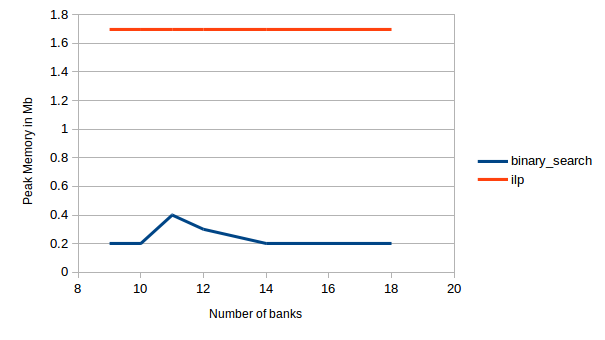
\includegraphics[width=12cm,height=7cm]{Taskset1.png}
}
\caption{Peak memory plot on Taskset I by Binary Search vs ILP}
\end{figure}

\begin{figure} [!htb]
%\label{fig1}
\centering
\fbox{
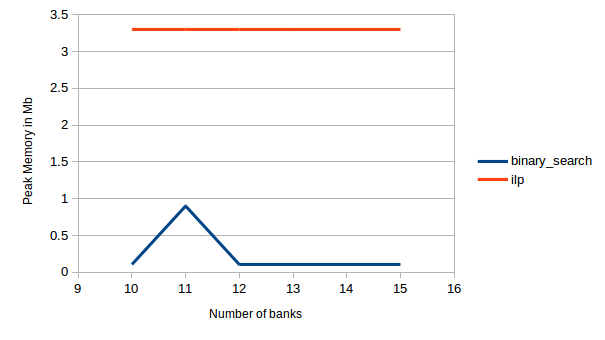
\includegraphics[width=12cm,height=7cm]{Taskset2.png}
}
\caption{Peak memory plot on Taskset II by Binary Search vs ILP}
\end{figure}

\begin{figure}
%\label{fig1}
\centering
\fbox{
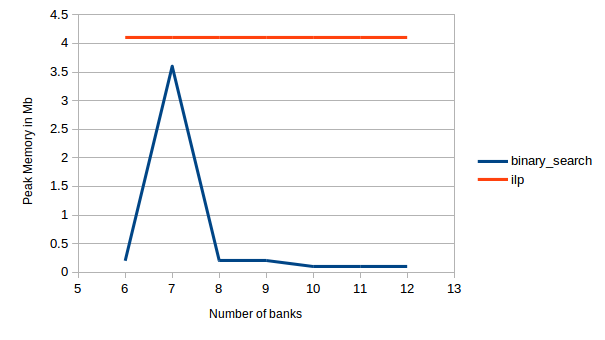
\includegraphics[width=12cm,height=7cm]{Taskset3.png}
}
\caption{Peak memory plot on Taskset III by Binary Search vs ILP}
\end{figure}


\begin{table}[t]
\centering
  \begin{tabular}{|c|c|c|c|c|}\hline
  {\bf Task} & {\bf Criticality} & {\bf Parallel} & {\bf Percentage of} & {\bf Deadline} \\  
  {\bf ID} & {\bf Level} & {\bf Bank access} & {\bf task executed} &              \\ \hline
    1 & L1 & 2 & 15\% & 10 cycles \\
      & L2 & 4 & 24\% &  \\
    2 & L1 & 1 & 10\% & 7 cycles \\
      & L2 & 3 & 15\% &          \\
      & L3 & 5 & 20\% &          \\
    3 & L1 & 2 & 15\% & 8 cycles \\
      & L2 & 3 & 20\% &          \\
      & L3 & 7 & 25\% &          \\
      & L4 & 8 & 30\% &          \\
    4 & L1 & 4 & 12\% & 7 cycles \\
      & L2 & 5 & 25\% &          \\
    5 & L1 & 2 & 10\% & 9 cycles \\
      & L2 & 4 & 12\% &          \\
      & L3 & 7 & 18\% &          \\
    6 & L1 & 3 & 15\% & 12 cycles \\
      & L2 & 5 & 20\% &           \\
      & L3 & 7 & 30\% &           \\ \hline      
  \end{tabular}
 \caption{Taskset I}
 \end{table}

\begin{table}[t]
\centering
  \begin{tabular}{|c|c|c|c|c|c|}\hline
  {\bf Task} & {\bf Criticality} & {\bf Parallel} & {\bf Percentage of} & {\bf Deadline} & {\bf Minimum number}\\  
   {\bf ID} & {\bf Level} & {\bf Bank access} & {\bf task executed} &             & {\bf of banks}\\ \hline
    1 & L1 & 3 & 18\% & 8 cycles & \\
      & L2 & 5 & 25\% &          & \\
    2 & L1 & 4 & 21\% & 6 cycles & \\
      & L2 & 5 & 26\% &          & 12 banks \\
      & L3 & 6 & 32\% &          & \\
    3 & L1 & 3 & 6\% & 7 cycles & \\
      & L2 & 6 & 13\% &         & \\
      & L3 & 8 & 17\% &         & \\
      & L4 & 9 & 25\% &         & \\ \hline    
 \end{tabular}
 \caption{Taskset II}
\end{table}


\begin{table}[t]
\centering
  \begin{tabular}{|c|c|c|c|c|c|}\hline
  {\bf Task} & {\bf Criticality} & {\bf Parallel} & {\bf Percentage of} & {\bf Deadline} & {\bf Minimum number}\\  
   {\bf ID} & {\bf Level} & {\bf Bank access} & {\bf task executed} &             & {\bf of banks}\\ \hline
   1 & L1  & 4 & 15\% & 10 cycles & \\
     & L2 & 6 & 30\% &            & \\
   2 & L1 & 2 & 22\% & 10 cycles & \\
     & L2 & 5 & 30\% &           & \\
   3 & L1 & 3 & 18\% & 10 cycles & 8 banks \\
     & L2 & 7 & 23\% &           & \\
   4 & L1 & 3 & 15\% & 10 cycles & \\
     & L2 & 5 & 21\% &           & \\ \hline    
   \end{tabular}
   \caption{Taskset III}
   \end{table}

 
